\section{Cilindretti}

\subsection{Descrizione della procedura di misura}
Procediamo ora con la descrizione della procedura operativa con cui
abbiamo misurato i 25 cilindri di metallo con i tre strumenti di
misura a nostra disposizione:

\subsubsection{Metro a nastro}
Abbiamo misurato i 25 cilindretti con un metro a nastro la cui risoluzione
di misura è 1 millimetro, in quanto abbiamo ritenuto di non poter distinguere
un intervallo di mezzo millimetro. Per questo motivo abbiamo approssimato
le misure alla tacca da un millimetro più vicina al bordo del cilindretto.
Poichè la lunghezza dei cilindretti era di circa 15 mm abbiamo incontrato
delle difficoltà nell'allineare i cilindri con lo 0 dello strumento.
Per questo motivo abbiamo allineato un'estremità di ogni cilindro con la
tacca dei 10 cm del metro e abbiamo sottratto questa quantità al valore
della misurà così ottenuta. E' importante evidenziare che anche in questa
operazione abbiamo riscontrato una certa difficoltà nell'allineare correttamente
i cilindri anche con la tacca dello strumento, ma ci è sembrato che la
misura così ottenuta fosse più precisa di quella riscontrata allineandoli
con lo 0 dello strumento. Ciò nonostante abbiamo tentato di evitare
eventuali errori di parallasse durante la lettura dello stumento.

\subsubsection{Calibro ventesimale}
Il calibro che abbiamo utillizzato ha una risoluzione di misura di 0.05
millimetri. La misura con il calibro ventesimale è stata effettuata avendo
cura di disporre i cilindri in modo perpendicolare ai becchi del calibro,
a tal fine abbiamo sfruttato le scanalature presenti sullo strumento.
In questo modo abbiamo tentato di misurare l'asse del cilindro, tuttavia
non abbiamo potuto evitare nella maniera più assoluta errori di posizione
dei cilindri.
La lettura dei ventesimi di millimetro è stata effettuata cercando quale
tacca della scala mobile ventesimale si allineasse meglio con le tacce
sovrastanti della scala millimetrata. Questa operazione è stata eseguita
da tutti i membri del gruppo per evitare eventuali problemi di parallasse
dovuti ad una singola valutazione della misura.

\subsubsection{Micrometro}
Il micrometro è uno strumento con una risoluzione di misura di 0.01
millimetro. Anche in questo caso la misura dei cilindri è stata effettuata
prestando attenzione che i campioni fossero perpendicolari alle aste di
misurazione, per evitare lo stesso tipo di errore descritto sopra.
Come nel caso del calibro non possiamo essere sicuri del perfetto
allineamento dei cilindri, ma abbiamo tentato di ridurre al minimo
questa problematica.

\begin{table}[tb]
	\footnotesize
	\centering
	\begin{tabular} { c c c c c | c c c c c | c c c c c }
		\toprule
		\multicolumn{15}{c}{Lunghezza dei cilindretti} \\
		\multicolumn{5}{c}{Metro [mm]} & \multicolumn{5}{c}{Calibro [mm]} & \multicolumn{5}{c}{Micrometro [mm]} \\
		\midrule
		14 & 14 & 14 & 14 & 14 & 13.70 & 13.85 & 13.95 & 13.80 & 13.95 & 13.94 & 13.92 & 13.84 & 13.93 & 13.79 \\
		14 & 14 & 14 & 14 & 14 & 13.70 & 13.95 & 13.90 & 13.90 & 13.90 & 13.94 & 13.93 & 13.89 & 13.92 & 13.91 \\
		14 & 14 & 14 & 14 & 14 & 13.70 & 13.95 & 13.90 & 13.95 & 13.85 & 13.93 & 13.93 & 13.84 & 13.90 & 13.74 \\
		14 & 14 & 14 & 14 & 14 & 13.70 & 13.95 & 13.90 & 13.90 & 13.90 & 13.70 & 13.85 & 13.91 & 13.79 & 13.70 \\
		13 & 14 & 14 & 14 & 14 & 13.75 & 13.90 & 13.80 & 13.85 & 13.90 & 13.71 & 13.92 & 13.91 & 13.94 & 13.70 \\
	\bottomrule
	\end{tabular}
	\caption{Misure della lunghezza dei 25 cilindretti ottenute con i tre strumenti a nostra disposizione.
        È riportato il valore di lettura degli strumenti.}
	\label{tab:cilindretti}
\end{table}

\subsection{Analisi dei dati}

\subsubsection{Dati raccolti con il metro}

La seguente tabella \ref{tab:cilindretti} riporta tutte le 25 misure di
lunghezza dei cilindri effettuate con ognuno dei tre strumenti a nostra
disposizione:

L'istogramma in figura \ref{fig:metro} rappresenta la distribuzione della lunghezza della
popolazione dei cilindretti ottenuta con il metro a nastro. Per costruire
questo istogramma abbiamo deciso di utilizzare come binnaggio la risoluzione
di misura dello strumento e quindi di 1 millimetro, poichè tutte le misure
effettuate sono risultate essere 14 $\pm$ 0.5 mm tranne una che ha valore
13 $\pm$ 0.5 mm. Come si può osservare dal grafico non siamo riusciti ad
apprezzare la distribuzione non uniforme della lunghezza dei cilindri,
in quanto la risoluzione dello strumento non è stata sufficiente per
apprezzare le variazioni di lunghezza da un corpo all'altro.

\begin{SCfigure}[0.6][bt]
	\centering
	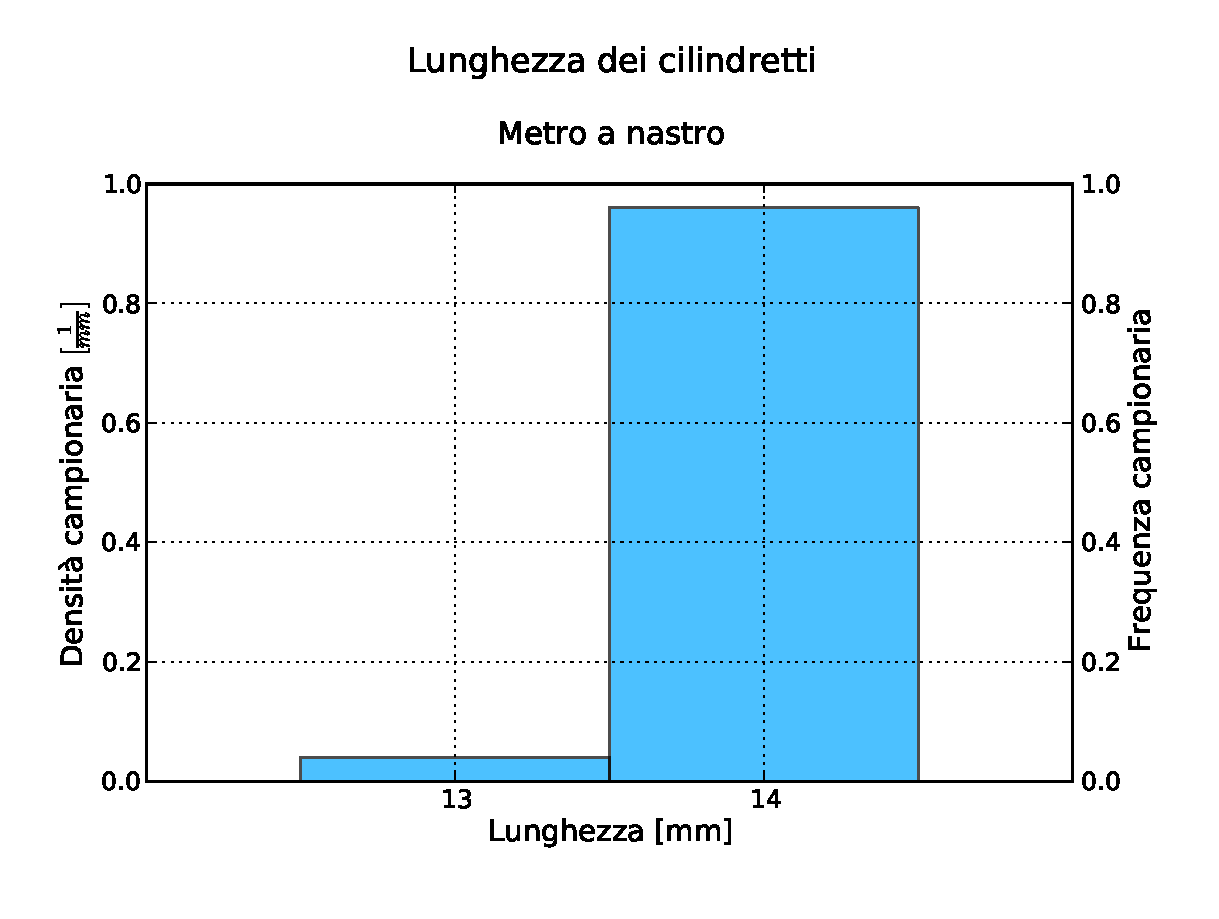
\includegraphics[width=100mm]{grafici/Cilindretti_metro.pdf}
	\caption{Istogramma relativo alle misure di lunghezza dei cilindri effrttuate con il
        metro a nastro. Come si può vedere chiaramente i dati sono dominati dall'errore di
        risoluzone dello strumento, che è inadatto per questo esperimento.}
	\label{fig:metro}
\end{SCfigure}

I parametri statistici ottenuti relativi alle misure dei cilindri sono
i seguenti:

% se vuoi elenco numerato sostituisci enumerate al posto di itemize
% ovviamente devi cambiare anche \end{itemize}
\begin{itemize}
    \item{Media campionaria:}
        \begin{equation}
        m^*[x] = \frac{1}{N} \sum_{i=1}^{N} (x_i) \simeq \sum_{j=1}^{\mathcal{N}} (x_j p_j^*) = 13.96\,\,mm 
        \end{equation}

    \item{Varianza campionaria:}
        \begin{equation}
        \tilde{D} = \frac{1}{N - 1} \sum_{i=1}^{N} (x_i - m^*[x])^2 = 0.04\,\,mm^2
        \end{equation}

    \item{Deviazione standard campionaria:}
        \begin{equation}
        \tilde{\sigma} = \sqrt{\frac{1}{N - 1} \sum_{i=1}^{N} (x_i - m^*[x])^2} = 0.2\,\,mm
        \end{equation}
\end{itemize}

Possiamo concludere dicendo che il valore di deviazione standard trovato non ha
senso, poiché è molto minore all'errore di risoluzione. Il metro non è
uno strumento adatto per compiere queste misure; infatti l'errore di risoluzione domina su
tutte le altre cause di incertezza, impedendo di ottenere risultati significativi
dall'esperimento.

\subsubsection{Dati raccolti con calibro e micrometro}

Gli istogrammi figura \ref{fig:calmic} rappresentano rispettivamente la distribuzione delle
misure della lunghezza dei cilindri ottenute con il calibro ventesimale e con
il micrometro.

\begin{wrapfloat}{figure}{r}{0pt}
	\centering
	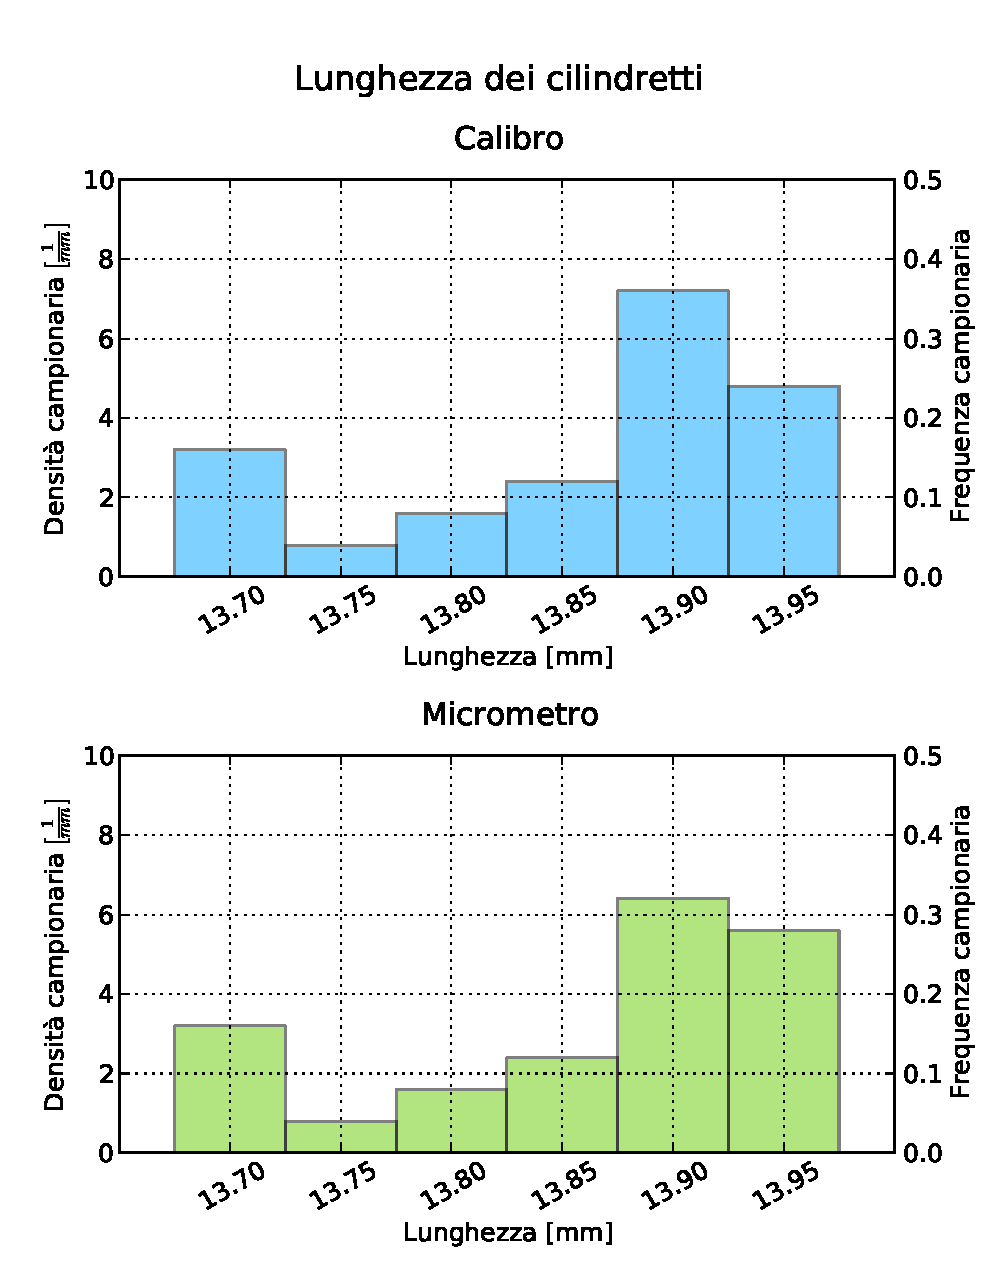
\includegraphics[width=100mm]{grafici/Cilindretti_calibro_micrometro.pdf}
	\caption{I due grafici riportano le lunghezze dei cilindri, misurati con calibro
        ventesimale e micrometro. Come si può notare i grafici sono identici a parte
        le ultime due colonne, dove un dato "ha cambiato" bin.}
	\label{fig:calmic}
\end{wrapfloat}

Per l'istogramma relativo al calibro ventesimale la scelta del binning è legata
alla risoluzione dello strumento e quindi la larghezza di ogni singolo
bin è di 0.05 mm. I dati sono infatti abbastanza numerosi per avere un numero
di conteggi sufficienti per ogni colonna.

Per l'istogramma relativo al micrometro, invece, si è scelto di utilizzare lo stesso
binnaggio utilizzato per il calibro. Abbiamo effettuato questa scelta poiché se avessimo
diminuito la larghezza dei bin avremmo ottenuto un numero di colonne troppo alto e per
ognuna di esse un numero di conteggi insufficiente. Al contrario se avessimo scelto
di aumentare la larghezza dei bin allora lo scopo di misurare i 25 cilindretti
con il micrometro sarebbe risultato vano in quanto non si sarebbe nemmeno apprezzata
la buona risoluzione dello strumento. D'altra parte questa scelta rende i grafici 
confrontabili direttamente.

Come si può notare i due istogrammi si assomigliano: infatti in entrambi i casi
siamo riusciti ad apprezzare la presenza di un picco della popolazione in
corrispondenza del valore 13.90 mm. La distribuzione dei cilindretti è stabile
nei due istogrammi ottenuti con strumenti diversi, a parte le ultime due colonne
che sono leggermente diverse. C'è un buon accordo tra le misure effettuate con
calibro e micrometro.

Tuttavia, nonostante le misure risultino essere
più accurate rispetto a quelle eseguite con il metro a nastro e la risoluzione
degli strumenti usati sia adeguata, non ci sono abbastanza campioni per poter affermare
l'esistenza di due popolazioni distinte di cilindretti, come sembra suggerire la colonna
centrata in (13.70 mm). Affermiamo questo perchè, considerando l'incertezza delle colonne,
la colonna si confonde con la coda del picco principale.

L'errore su ogni colonna è $\sqrt{n_j}$, dove $n_j$ è il numero di dati che cadono nel
bin $j$-esimo. Il conteggio della prima colonna (quella centrata in 13.70 mm) è $n_1 = 4$,
la sua incertezza è $\sqrt{4} = 2$, mentre la seconda colonna (centrata in 13.75 mm) ha un
solo conteggio $n_2 = 1$, con errore uguale a 1. Tenendo conto di questo, gli intervalli
di incertezza delle colonne si toccano, e quindi la prima colonna può semplicemente essere
una fluttuazione casuale della coda.

Più nel dettaglio possiamo dire che i dati statistici riguardanti le misure con il calibro
ventesimale e il micrometro sono:

\begin{itemize}
    \item{Media campionaria:}
        \begin{equation*}
        m^*_{cal}[x] \simeq 13.86\,\,mm \qquad
        m^*_{mic}[x] \simeq 13.86\,\,mm 
        \end{equation*}

    \item{Varianza campionaria:}
        \begin{equation*}
        \tilde{D}_{cal} = 0.0077\,\,mm^2 \qquad
        \tilde{D}_{mic} = 0.0076\,\,mm^2
        \end{equation*}

    \item{Deviazione standard campionaria:}
        \begin{equation*}
        \tilde{\sigma}_{cal} = 0.09\,\,mm \qquad
        \tilde{\sigma}_{mic} = 0.09\,\,mm
        \end{equation*}
\end{itemize}

Come già notato sopra, le misure effettuate con calibro e micrometro sono compatibili.
I valori medi campionari delle lunghezze e le deviazioni tipo campionarie sono
uguali per entrambi gli strumenti.

Altri parametri statistici includono:

\begin{itemize}
    \item{Mediana:}
        \begin{equation*}
        m_{cal}[x] \simeq 13.90\,\,mm \qquad
        m_{mic}[x] \simeq 13.91\,\,mm 
        \end{equation*}

    \item{Quantile 10\%:}
        \begin{equation*}
        q_{10\%cal} = 13.70\,\,mm \qquad
        q_{10\%mic} = 13.70\,\,mm
        \end{equation*}

    \item{Quantile 90\%:}
        \begin{equation*}
        q_{90\%cal} = 13.95\,\,mm \qquad
        q_{90\%mic} = 13.94\,\,mm
        \end{equation*}
\end{itemize}
% Inserire oltre  a Media campionaria, Varianza campionaria, Fluttuazione standard
% campionaria anche mediana e quantili
% Ulteriori commenti

\begin{SCfigure}[][p]
	\centering
	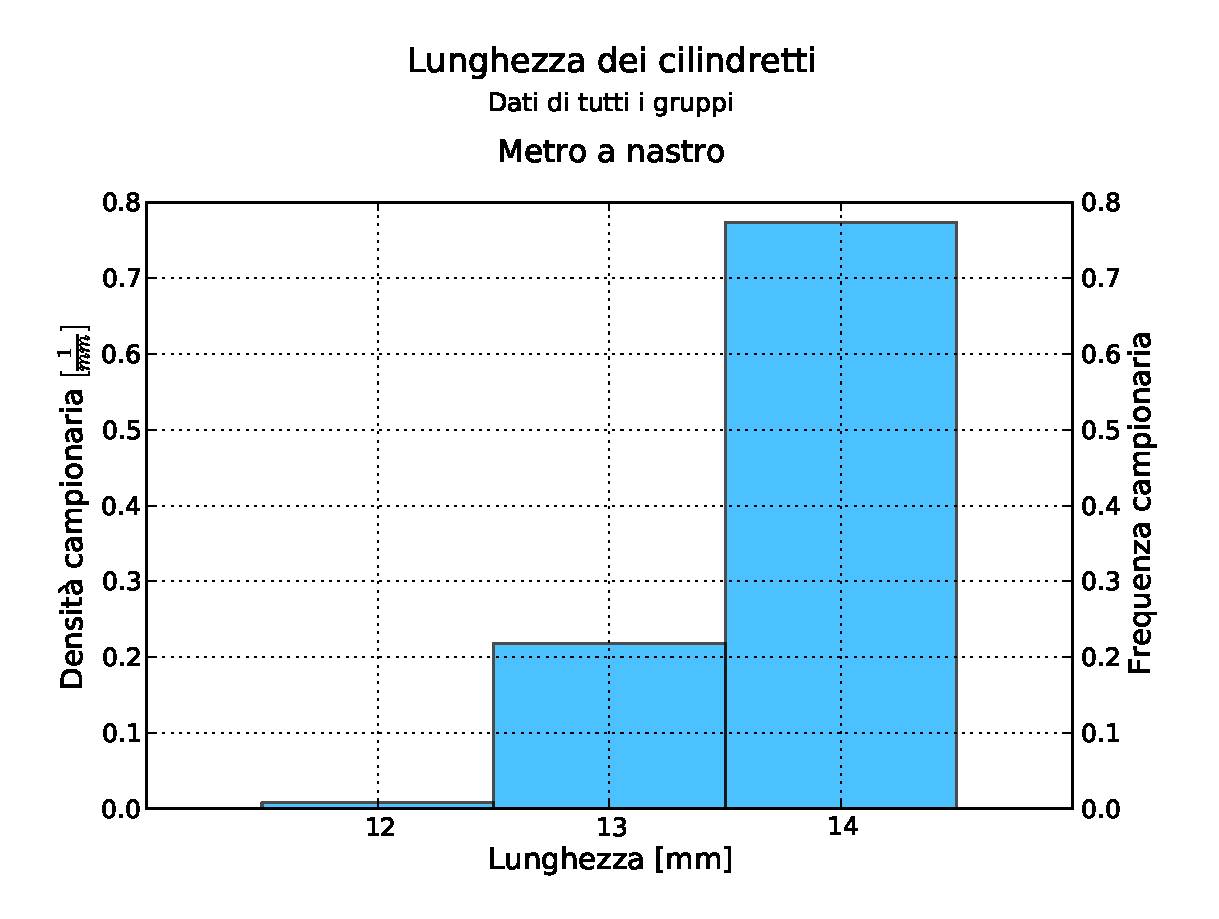
\includegraphics[width=100mm]{grafici/cilindri_tutti.pdf}
	\caption{Misure della lunghezza dei cilindretti ottenute da tutti i gruppi del
        laboratorio (gruppi del lunedì). L'istogramma riporta le misure effettuate con
        il metro a nastro. Come si può vedere la risoluzione dello strumento è
        insufficiente per fare una qualsiasi analisi qualitativa dei dati ottenuti.}
    \label{fig:metro_tutti}
\end{SCfigure}

\begin{SCfigure}[][p]
	\centering
	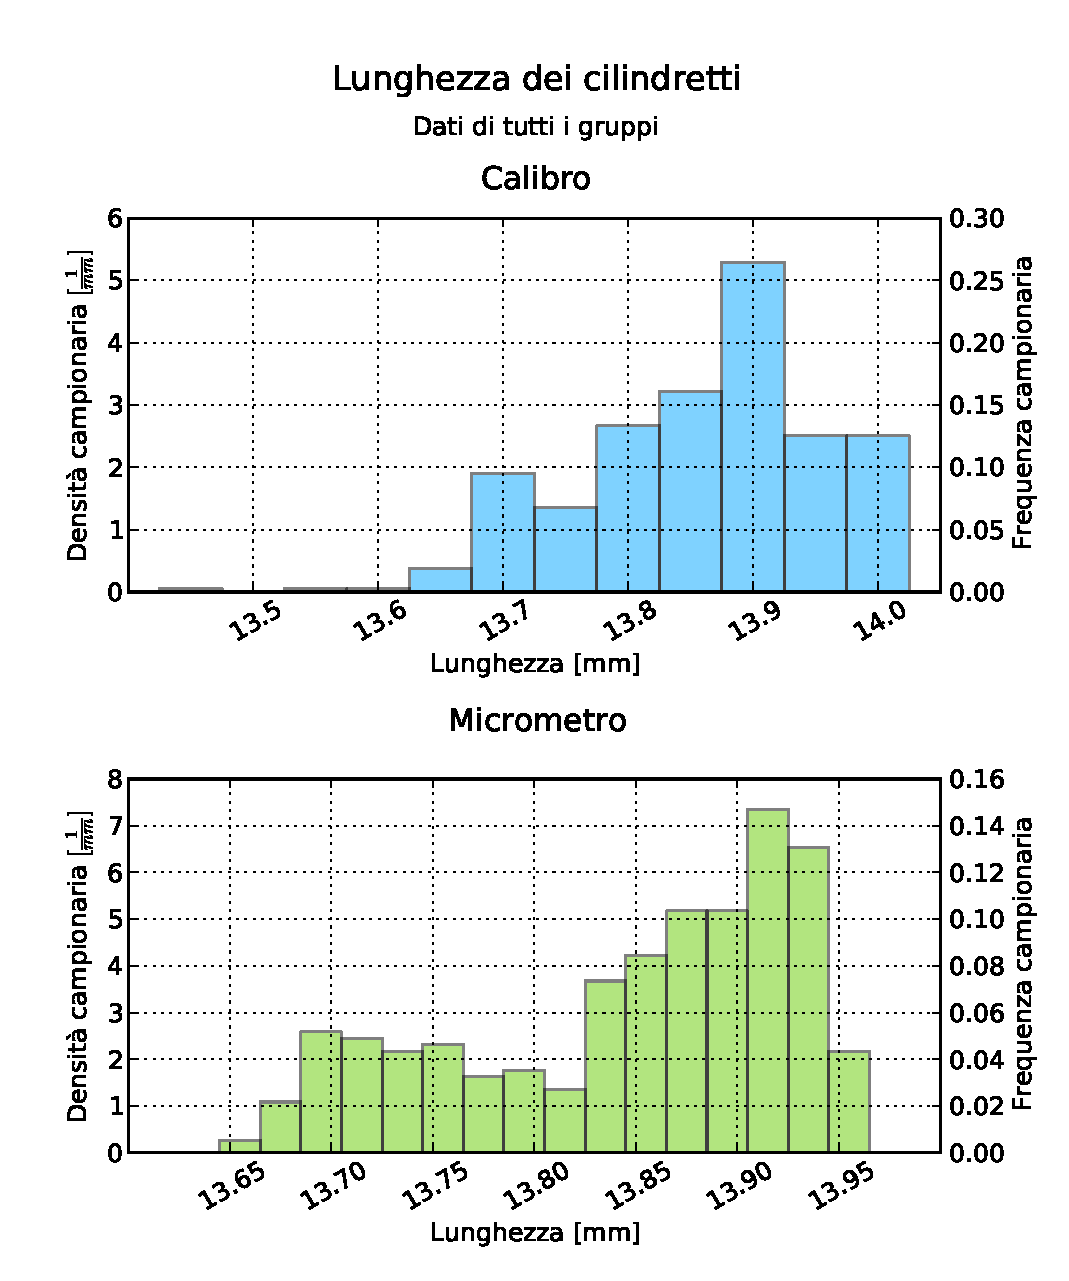
\includegraphics[width=100mm]{grafici/cilindri_tutti_2.pdf}
    \caption{Lunghezza dei cilindretti ottenute da tutti i gruppi (del lunedì)
        del corso di laboratorio. L'istogramma relativo alle misure con il calibro
        ha binning di 0.05 mm, mentre nell'istogramma delle misure effettuate con
        il micrometro i bin sono da 0.02 mm. Si può notare con facilità, nel grafico
        delle misure con il micrometro, che esiste una seconda popolazione di
        cilindretti più corti che si distacca nettamente dalla coda del picco principale.
        Questa popolazione è molto meno visibile nel grafico relativo al calibro, dove si
        notano anche degli evidenti errori di misura.}
    \label{fig:calmic_tutti}
\end{SCfigure}

\subsection{Analisi dei dati a livello globale di laboratorio}

Oltre all'analisi dei dati raccolti dal gruppo, abbiamo analizzato anche i dati
ottenuti dagli altri gruppi del lunedì. Non abbiamo informazioni per quanto riguarda
gli errori sistematici commessi in quanto le misure non sono state raccolte
da noi e siamo ignoranti per quanto riguarda le modalità di acquisizione.
Ci limiteremo ad un'analisi della forma dell'istogramma e al calcolo dei parametri
statistici principali.

I dati ottenuti sono mostrati negli istogrammi delle figure \ref{fig:metro_tutti} e \ref{fig:calmic_tutti}.
Le tabelle dei dati non sono riportate per motivi di spazio; avevamo infatti 367 misure differenti.

\subsubsection{Dati misurati col metro}

Come sopra, i dati raccolti con il metro a nastro non ci permettono
di affermare nulla sulla natura dei cilindri, in quanto la risoluzione dello strumento
è ampiamente insufficiente allo scopo. Questo è evidente dal grafico e per
questo motivo non ci dilungheremo oltre sull'argomento.

\subsubsection{Dati misurati con calibro e micrometro}

Contrariamente a quanto abbiamo potuto ricavare dai dati
raccolti dal nostro singolo gruppo con i tre strumenti, i dati relativi
a tutti i gruppi ci permettono di evidenziare l'esistenza di due popolazioni
distinte di cilindri.

Queste due popolazioni non sono distinguibili nell'istogramma riguardante il calibro
in figura \ref{fig:calmic_tutti}. Potrebbe sembrare che la colonna centrata
in 13.70 mm si distacchi dalla coda del picco, ma come sopra, procediamo a dimostrare
che in realtà potrebbe essere dovuta a fluttuazioni causali.
Nel bin centrato in 13.70 mm cadono 35 misure, mentre nel bin accanto (13.75 mm) ne cadono 25.
Gli errori sulle colonne sono rispettivamente $\sqrt{35} \simeq 6$ e $\sqrt{25} = 5$.
Gli intervalli di incertezza si toccano e per questo la colonna si può considerare
una fluttuazione.

Nel secondo istogramma in figura \ref{fig:calmic_tutti} invece, sono ben distinguibili due picchi,
che corrispondono alle due diverse popolazioni di cilindretti. Anche in questo caso in realtà,
tenendo conto delle incertezze sulle colonne, le colonne si confondono. Tuttavia
la deviazione dalla coda è ben accentuata in diversi bin e quindi possiamo ragionevolmente 
supporre l'esistenza di due popolazioni distinte di cilindretti.

Evidentemente la risoluzione di misura è stata determinante per individuare le popolazioni.
I parametri statistici principali sono:

\begin{itemize}
    \item{Media campionaria}
    \begin{equation*}
        m^*_{cal}[x] \simeq 13.86\,\,mm \qquad
        m^*_{mic}[x] \simeq 13.85\,\,mm 
    \end{equation*}

    \item{Deviazione standard campionaria:}
    \begin{equation*}
        \tilde{\sigma}_{cal} = 0.10\,\,mm \qquad
        \tilde{\sigma}_{mic} = 0.08\,\,mm
    \end{equation*}
\end{itemize}

Come si può facilmente vedere, i dati sono tra loro compatibili poiché:

\begin{equation*}
    |R| := |m^*_{cal}[x] - m^*_{mic}[x]| = 0.01 \, mm
\end{equation*}

\begin{equation*}
    \sigma_{R} := \sqrt{\tilde{\sigma}_{cal}^2 + \tilde{\sigma}_{mic}^2} = 0.13 \, mm \\
\end{equation*}


\begin{equation*}
    |R| \leq \sigma_{R}
\end{equation*}
